\documentclass{article}
\usepackage{graphicx}
\usepackage{amsmath}
\usepackage{fancyhdr}
\usepackage[colorlinks=true, linkcolor=cyan, citecolor=cyan, urlcolor=green]{hyperref}
\pagestyle{fancy}
\lhead{Ali Abdollahi}
\rhead{Project 2}
\cfoot{Page \thepage}
\title{The Third Project\\\large Encoding \& Learning}
\begin{document}
	\maketitle
	\section{Encoding}
	Three encodings models were utilized in this project. Time to first spike, Poisson, and Positional coding. The 12 images were shown in the figure\ref{im}. All of the encoding functions, codes any image to a desired number of neurons and time. For down sampling the number of pixels, two methods were utilized. First, average and max pooling. And second, choosing a random sample of the pixels. 
	
	\begin{figure}[h]
		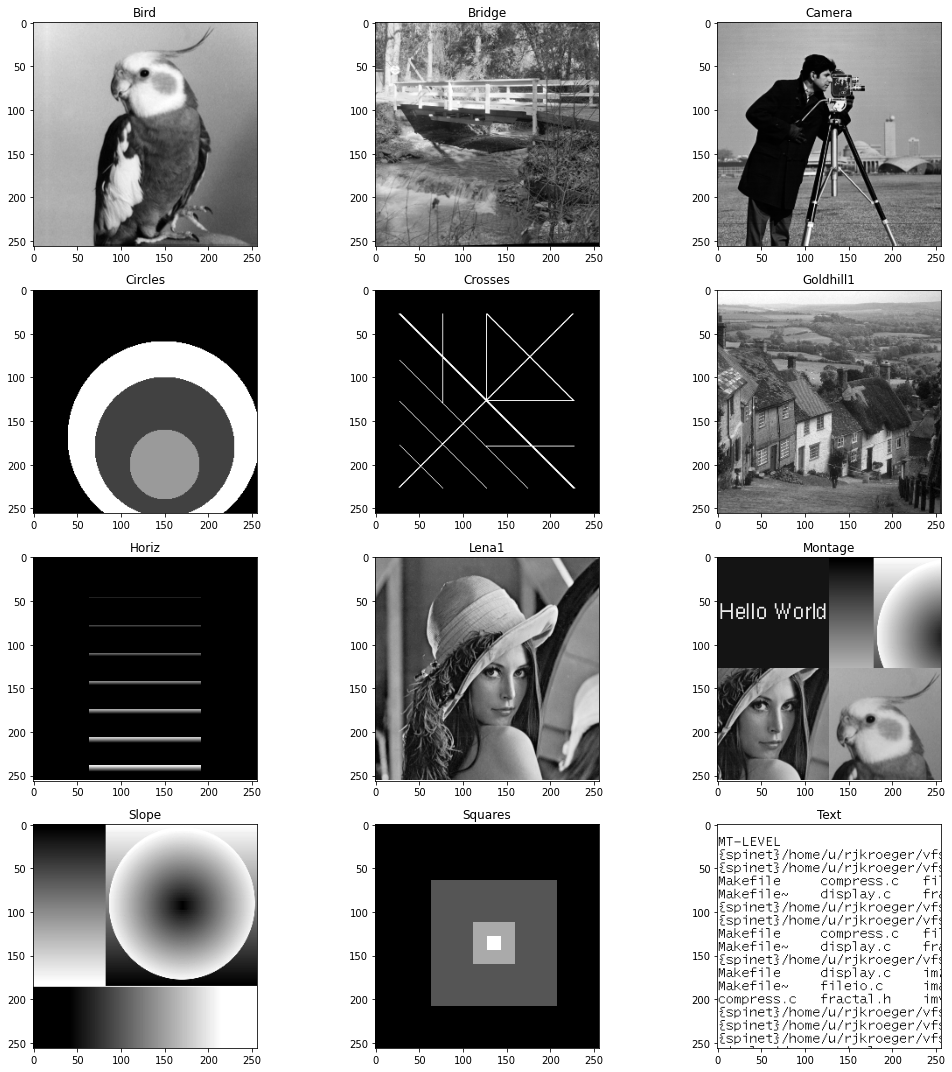
\includegraphics[width=1.2\textwidth]{images.png}
		\caption{The 12 images from this \href{https://links.uwaterloo.ca/Repository.html}{repository}, which used for encoding.}
		\label{im}
	\end{figure}
	\subsection{Time To First Spike}
	In the time to first spike method, only the first spike of each neuron matters. Thus, the coding is far sparser than the following encodings. These encodings are depicted in figure\ref{imttfs}.
	\begin{figure}[h]
		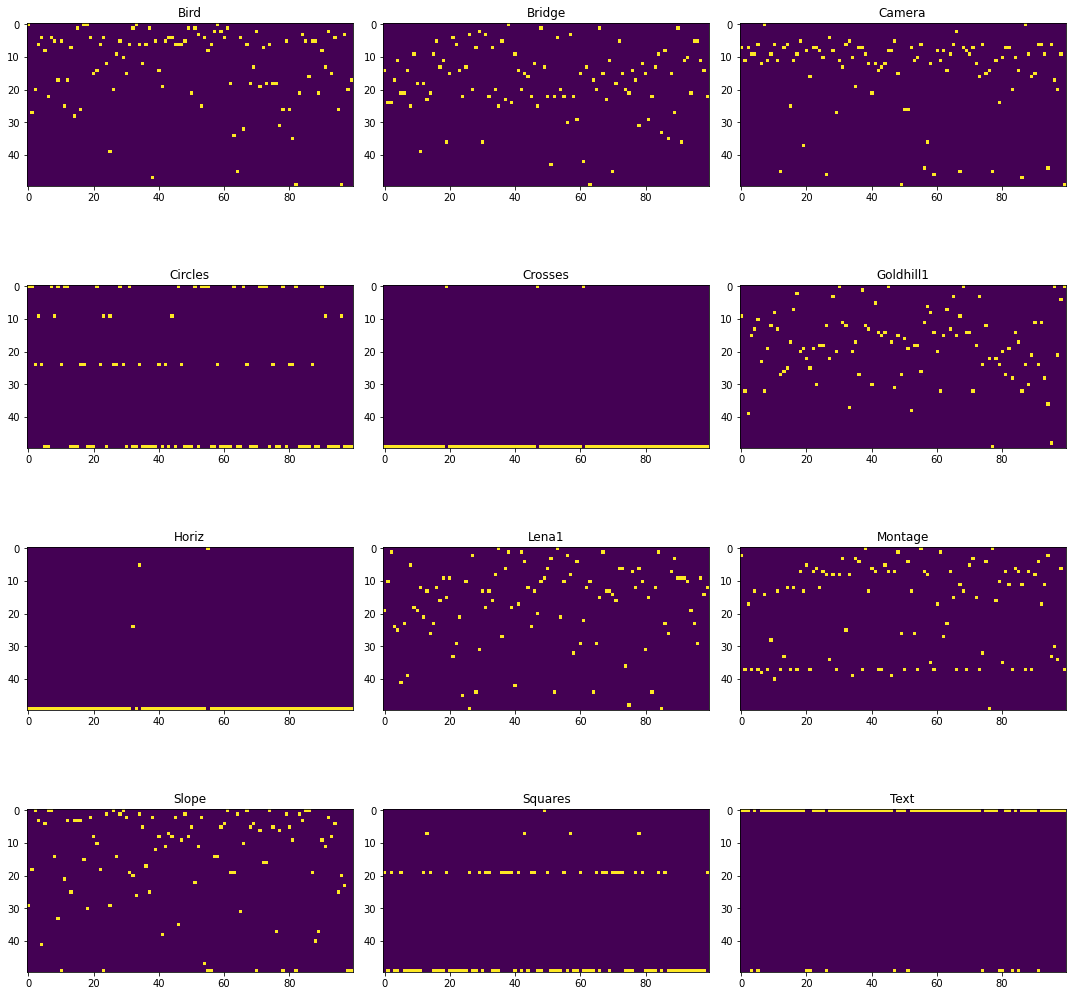
\includegraphics[width=1.2\textwidth]{images_ttfs.png}
		\caption{The TTFS encoding of the selected 12 images. The X-axis represents neurons and the Y-axis represents time}
		\label{imttfs}
	\end{figure}
	
	In the three of the images, crosses, text, and horiz, because most of the image is same and there is no complexity, the encodings are simple. For instance, in the crosses  and in the horiz, almost all of the neurons fires in the end, as most of the pixels are same. For circles and Squares, thanks to 4 spectrum of gray, there are 4 time steps where the corresponding neurons fire.
	\subsection{Poisson Coding}
	A random Poisson sample is generated for each value.
	
	\begin{figure}[h]
		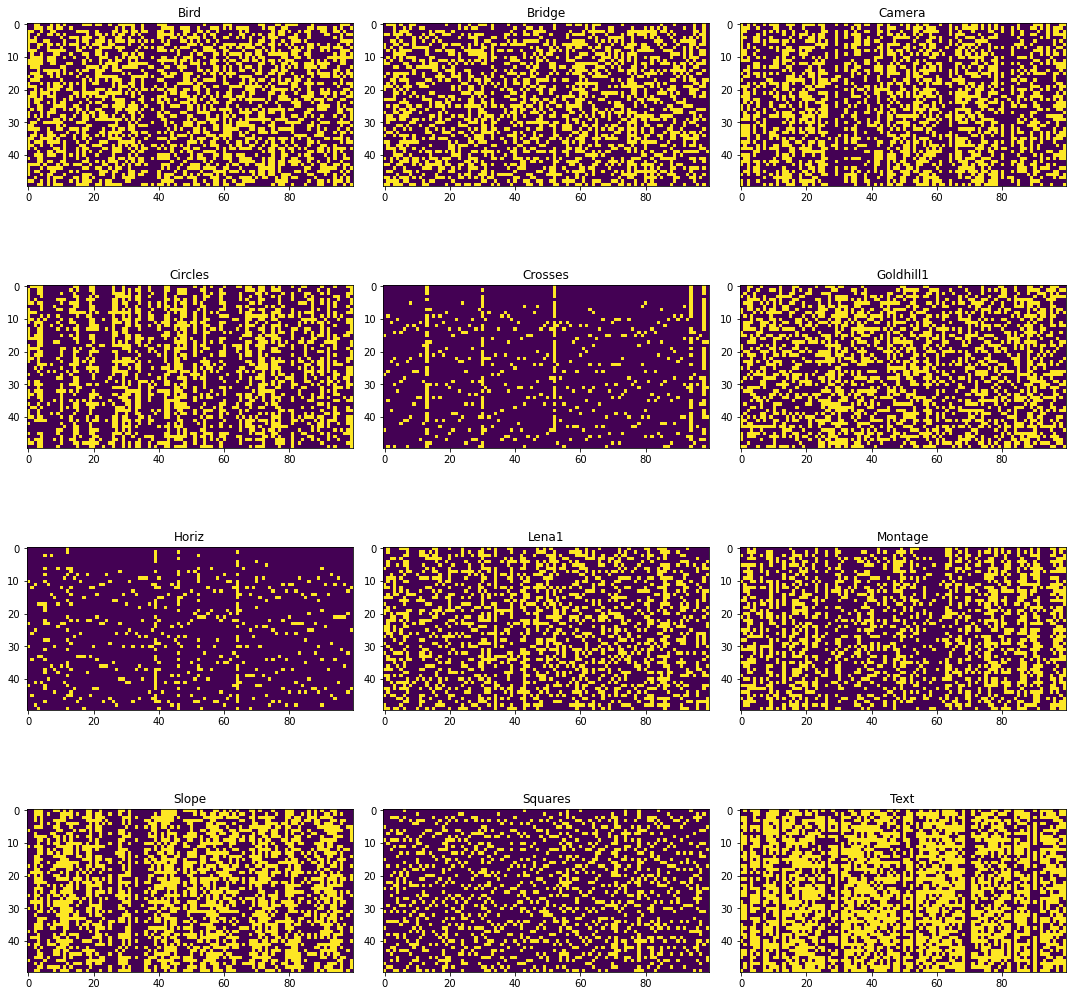
\includegraphics[width=1.2\textwidth]{images_poisson.png}
		\caption{The positional Coding of the images}
		\label{impois}
	\end{figure}
	
	As depicted in the plots, again for the crosses and the horiz, there is much less activity, because most of the pixels are 0. For text, that is the opposite case. For circles, we can observe that some neurons spikes much more frequent than other, which implies the different scale of grays.
	
	\subsection{Positional Values Coding}
	With this encoding, each pixel corresponds to a number of neurons. Each of those, denotes a different Gaussian plot. Their means are scattered in the range of pixels, typically 256 ($ [0, 1]$ if pixels were normalized), and the neurons fire with respect to the point which the desired value line intersects it. Thus, the closer the value to the mean, the earlier it fires (or if desired, the later it fires). 
	
	For efficiency, we did not compute all the neurons' probability density function (PDF). But rather the closest neuron is calculated, and the the nearest three from right and left were participated in this operation. Therefore, instead of calculating the PDF for $N$ normal distributions, only a small number (in our experiment 6) were selected.
	
	\begin{figure}[h]
		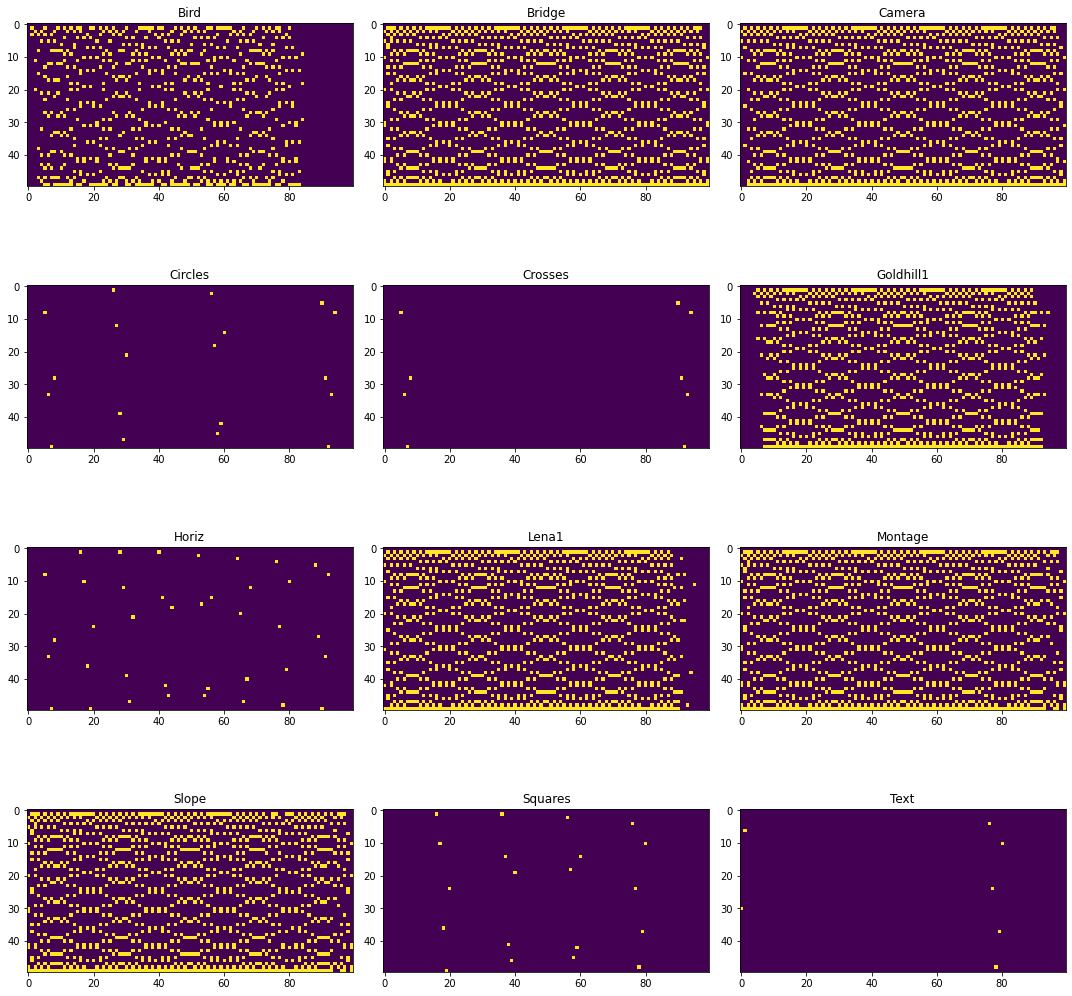
\includegraphics[width=1.2\textwidth]{images_pos.png}
		\caption{The positional Coding of the images}
		\label{impos}
	\end{figure}
	
	\section{STDP}
\end{document}
